\documentclass[12pt, twoside]{article}
\usepackage[letterpaper, margin=1in, headsep=0.5in]{geometry}
\usepackage[english]{babel}
\usepackage[utf8]{inputenc}
\usepackage{amsmath}
\usepackage{amsfonts}
\usepackage{amssymb}
\usepackage{tikz}
\usetikzlibrary{quotes, angles}
\usepackage{graphicx}
\usepackage{enumitem}
\usepackage{multicol}
\usepackage{hyperref}

\newif\ifmeta
\metatrue %print standards and topics tags

\title{IB Mathematics}
\author{Chris Huson}
\date{September 2021}

\usepackage{fancyhdr}
\pagestyle{fancy}
\fancyhf{}
\renewcommand{\headrulewidth}{0pt} % disable the underline of the header
\raggedbottom


\fancyhead[LE]{\thepage}
\fancyhead[RO]{\thepage \\ Name: \hspace{4cm} \,\\}
\fancyhead[LO]{BECA / IB Math 03-Quadratic functions\\* 6 January 2022}

\begin{document}

\subsubsection*{3.3 Graphing quadratic functions}
%Equations of a straight line: $f(x)=mx+c$, $ax+by+d=0$, $(y-y_1)=m(x-x_1)$\\[0.25cm]
%Gradient: $\displaystyle m=\frac{y_2-y_1}{x_2-x_1}$\\[0.25cm]
Useful forms of equations for quadratics:\\[0.25cm] 
$f(x)=ax^2 + bx+c$, with $y$-intercept $c$, axis of symmetry $\displaystyle x=-\frac{b}{2a}$, zeros $\displaystyle x=\frac{-b \pm \sqrt{b^2-4ac}}{2a}$\\[0.25cm]
$g(x)=a(x-p)(x-q)$, with $x$-intercepts $p$, $q$ and axis of symmetry $\displaystyle x=\frac{p+q}{2}$\\[0.25cm] 
$h(x)=a(x-h)^2+k$, with vertex $(h,k)$
\vspace{0.5cm}
\begin{enumerate}
\item   Given $f(x)=(x-1)(x-5)$
    \begin{enumerate}[itemsep=0.9cm]
        \item Write down the two solutions to $f(x)=0$. Mark them as the $x$-intercepts on the axes below.
        \item Expand the function to standard form, $f(x)=ax^2+bx+c \text{ where } a, b, c \;  \epsilon \; \mathbb{R}$. \vspace{2.5cm}
        \item Write down the value of $f(0)$. Mark it as the $y$-intercept on the graph.
        \item Sketch the function, labeling the vertex as an ordered pair. Show the axis of symmetry as a dotted line and label it with its equation.
        \begin{center}
            \begin{tikzpicture}
                \draw [thick, ->] (-4.5,0) -- (+4.5,0) node [right] {$x$};
                \draw [thick, ->] (0,-3.5) -- (0,4.5) node [left] {$y$};
            \end{tikzpicture}
            \end{center}
    \end{enumerate}

\newpage
\item The function $f(x)=-x^{2}+6x-7$ is shown on the graph.
\begin{enumerate}
  \begin{multicols}{2}
      \item Write down its vertex as an ordered pair. \vspace{0.5cm}
      \item Write down the domain and range of $f$. \vspace{1cm}
      \item Draw on the graph the function \\$g(x)=x-3$.
      \item Write down the two ordered pairs that satisfy both $f$ and $g$. \vspace{3cm}
      \begin{center}
      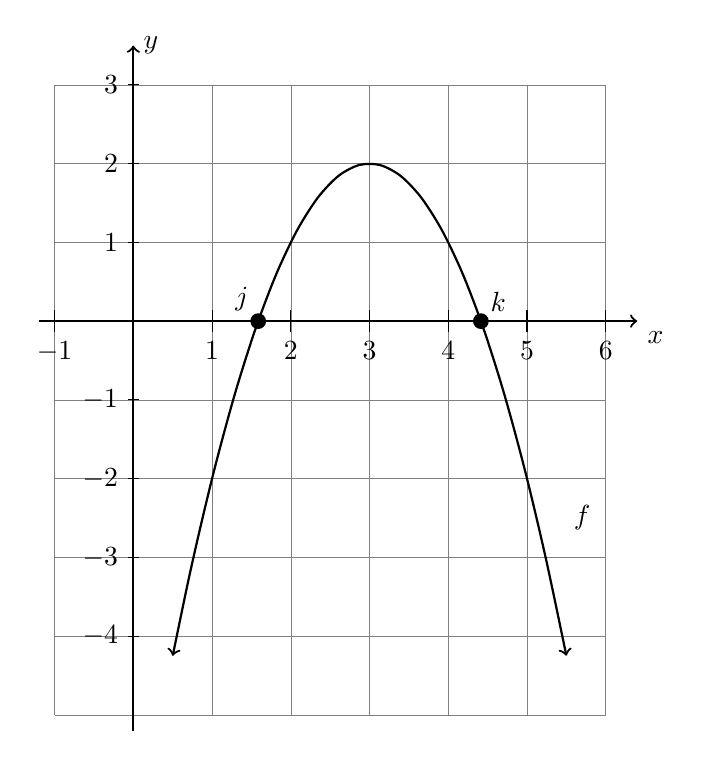
\begin{tikzpicture}[scale=1]
        \draw [help lines] (-1,-5) grid (6,3);
        \draw [thick, ->] (-1.2,0) -- (6.4,0) node [below right] {$x$};
        \draw [thick, ->] (0,-5.2)--(0,3.5) node [right] {$y$};

        \foreach \x in {-1, 1,2, ..., 6} \draw (\x cm,4pt) -- (\x cm,-4pt) node[below] {$\x$};

        \foreach \y in {-4,...,-1,1,2,..., 3} \draw (2pt,\y cm) -- (-2pt,\y cm) node[left] {$\y$};
        \fill (1.586,0) circle[radius=0.1] node[above left]{$j$};
        \fill (4.414,0) circle[radius=0.1] node[above right]{$k$};
        \draw [thick, <->,smooth,samples=20,domain=0.5:5.5] plot(\x,-\x*\x+6*\x-7);
        \node at (5.7,-2.5){$f$};
      \end{tikzpicture}
      \end{center}
    \end{multicols} 
    \vspace{0.5cm}
    \item Find the exact values of $j$ and $k$, the $x$-intercepts of $f$. (as an expression with radicals, not a decimal)
\end{enumerate} \vspace{3cm}

\newpage
\item Let $f$ be a quadratic function. Part of the graph of $f$ is shown below.\\*
The vertex is at $P(4,2)$ and the $y$-intercept is at $Q(0, 6)$.\\*
    \begin{center}
    \begin{tikzpicture}

        \foreach \x in {1,2,3,4,5,6}
        \draw (\x cm,3pt) -- (\x cm,-3pt) node[below] {$\x$};

        \foreach \y in {-1,1,2,3,4,5,6}
        \draw[shift={(0,\y)},color=black] (2pt,0pt) -- (-2pt,0pt) node[left]  {$\y$};
        \draw [thick, ->] (-2.5,0) -- (+6.5,0) node [right] {$x$};
        \draw [thick, ->] (0,-1.5) -- (0,6.5) node [right] {$y$};
        \fill (4,2) circle[radius=2pt] node [below] {$P$};
        \fill (0,6) circle[radius=2pt] node [right] {$Q$};
        \draw [<->] plot[domain= -0.25:6.5] (\x, .25*\x*\x -2*\x +6);
    \end{tikzpicture}
    \end{center}
    \begin{enumerate}[itemsep=1.5cm]
        \item Write down the equation of the axis of symmetry.
        \item Write down the domain and range of $f$.
        \item The function $f$ can be written in the form $f(x)=a(x-h)^2 +k$. \\*
        Write down the value of $h$ and of $k$.
        \item Find $a$.
    \end{enumerate}

\newpage
\item Consider the function $f(x)=ax^2 + bx+c$. The graph of $y=f(x)$ is shown in the diagram. The vertex of the graph has coordinates $(0.5, -12.5)$. The graph intersects the $x$-axis at the two points, $(-2,0)$ and $(p,0)$.
    \begin{flushright}
        \bf{diagram not to scale}
    \end{flushright}
        \begin{center}
        \begin{tikzpicture}[yscale=0.5]
            %\foreach \x in {-2, -1,1,2,3,4,5,6}
            %\draw[shift={(\x,0)},color=black] (0pt,-3pt) -- (0pt,3pt) node[below]  {$\x$};
            %\foreach \y in {-1,1,2,3,4,5,6}
            %\draw[shift={(0,\y)},color=black] (2pt,0pt) -- (-2pt,0pt) node[left]  {$\y$};
            \draw [thick, ->] (-2.5,0) -- (+4,0) node [right] {$x$};
            \draw [thick, ->] (0,-13) -- (0,1.5) node [left] {$y$};
    
            \fill (0.5,-12.5) ellipse(2pt and 4pt) node [below right] {$(0.5,-12.5)$};
            \fill (-2,0)  ellipse(2pt and 4pt) node [above left] {$(-2,0)$};
            \fill (3,0) ellipse(2pt and 4pt) node [above left] {$(p,0)$};
            \draw [<->] plot[smooth, domain= -2.25:3.25] (\x, 2*\x*\x -2*\x -12);
        \end{tikzpicture}
        \end{center}
        \begin{enumerate}
            \item Find the value of $p$. \vspace{2.5cm}
            \item Find the value of:
            \begin{enumerate}[itemsep=1cm]
                \item $a$.
                \item $b$.
                \item $c$.
            \end{enumerate}\vspace{1.5cm}
            \item Write down the equation of the axis of symmetry.
        \end{enumerate}

\newpage
\item Consider the function $f(x)=x^2+2x-3$.
    \begin{enumerate}
        \item Sketch the graph of $f$, for $-4 \leq x \leq 2$. Label the vertex and the intercepts.
        \item This function can also be written in the form $f(x)=(x-p)^2 -4$.\\* 
        Write down the value of $p$. \vspace{1.5cm}
        \item The graph of $f$ has two solutions for $f(x)=0$. Write down the solutions (or roots, zeros) of the function. \vspace{1.5cm}
        \item Hence, write down the function in factored form, $f(x)=(x-a)(x-b)$. \vspace{1.5cm}
    \end{enumerate}
    \begin{center}
    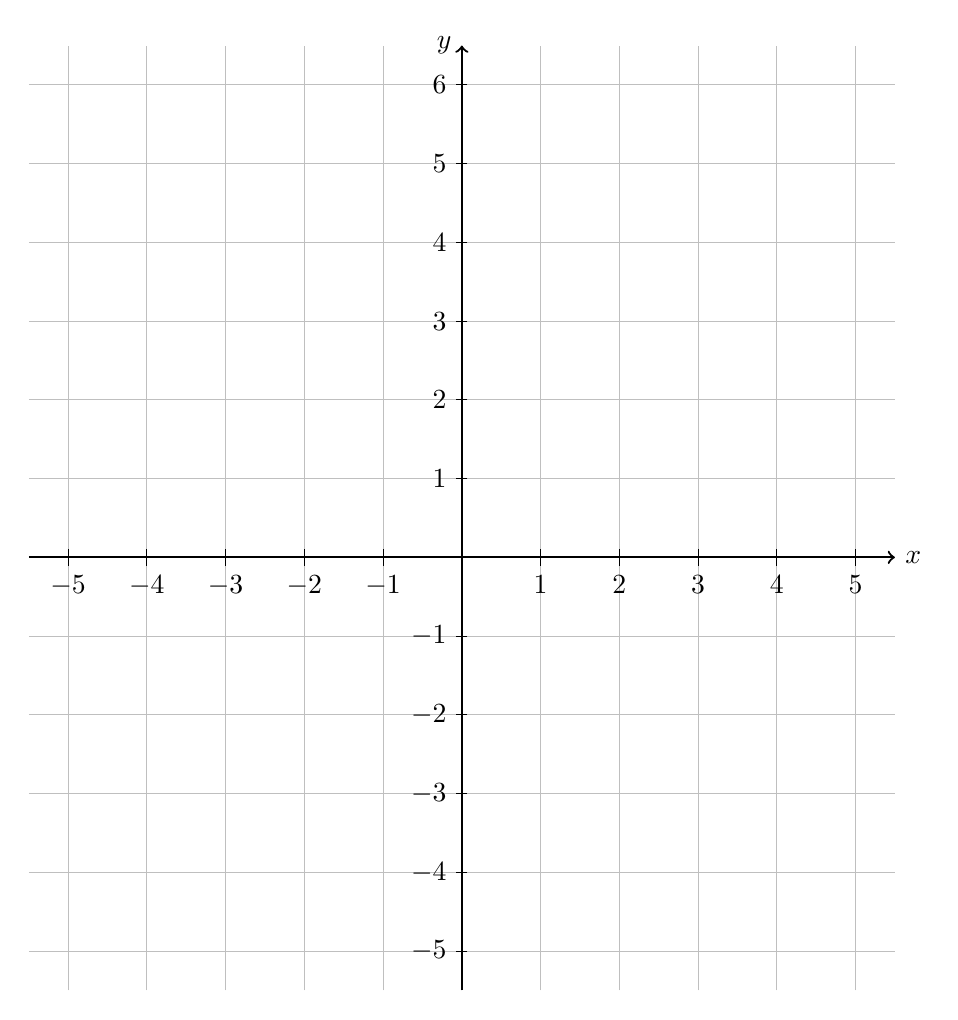
\begin{tikzpicture}
        \draw [thin, color=lightgray,, xstep=1.0cm,ystep=1.0cm] (-5.5,-5.5) grid (5.5,6.5);
        \foreach \x in {-5, -4, -3, -2, -1,1,2,3,4, 5}
        \draw (\x cm,3pt) -- (\x cm,-3pt) node[below] {$\x$};
        \foreach \y in {-5, -4, -3, -2, -1, 1,2,3,4, 5, 6}
        \draw[shift={(0,\y)},color=black] (2pt,0pt) -- (-2pt,0pt) node[left]  {$\y$};
        \draw [thick, ->] (-5.5,0) -- (+5.5,0) node [right] {$x$};
        \draw [thick, ->] (0,-5.5) -- (0,6.5) node [left] {$y$};
    \end{tikzpicture}
    \end{center}
\end{enumerate}
\end{document}